\section{Introduction}

Let's examine the configuration of a contemporary control system, as illustrated below:
\begin{figure}[H]
    \centering
    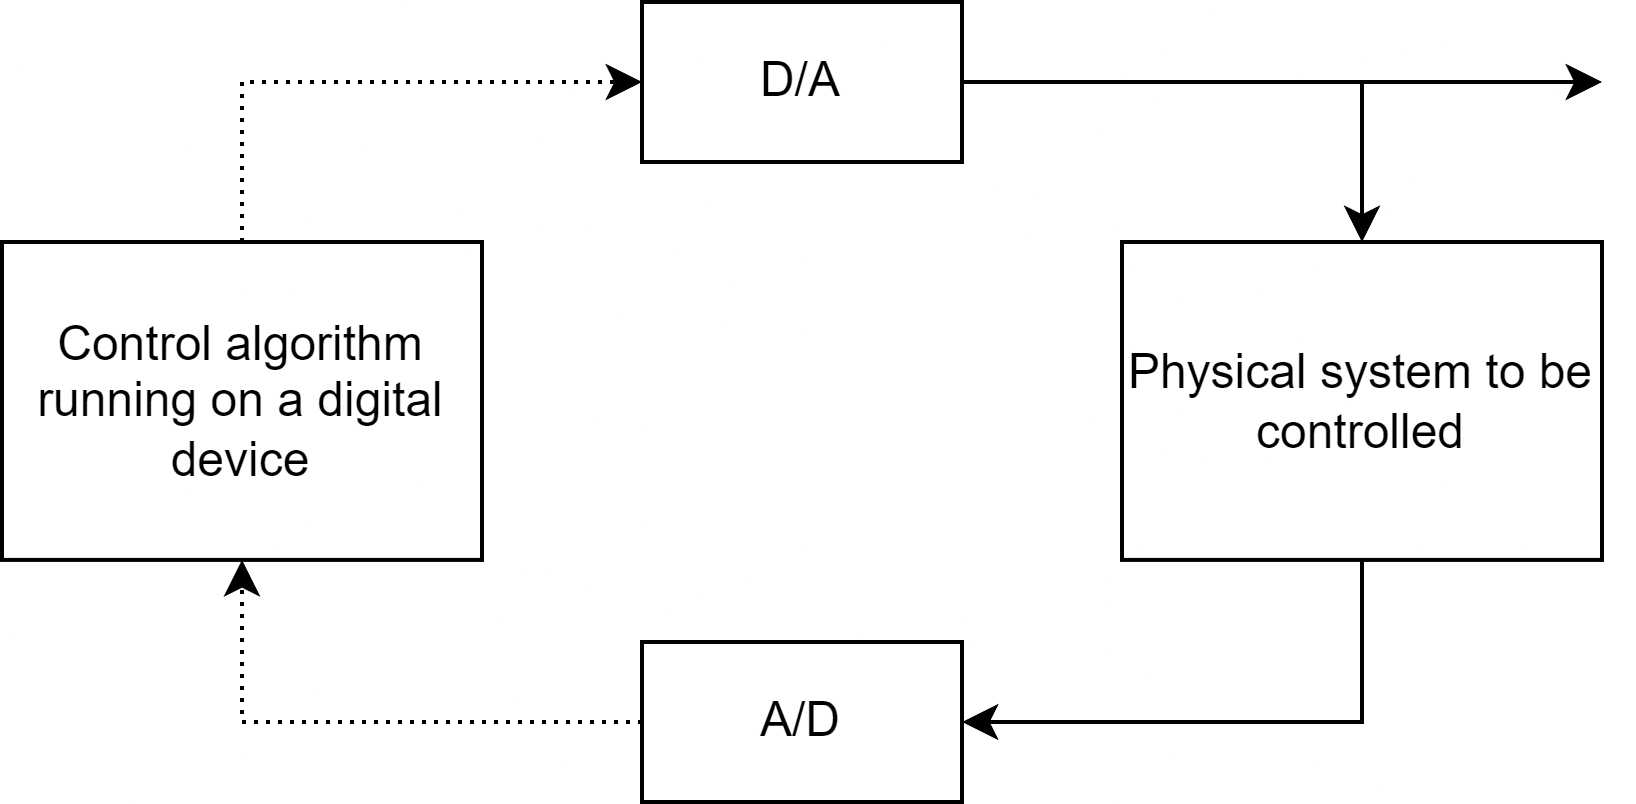
\includegraphics[width=0.5\linewidth]{images/discret.png}
    \caption{Physical system}
\end{figure}

\paragraph*{Analog to digital converter}
The analog to digital converter (ADC) facilitates the conversion of an analog signal into a discrete form, operating on both time and amplitude domains.
\begin{figure}[H]
    \centering
    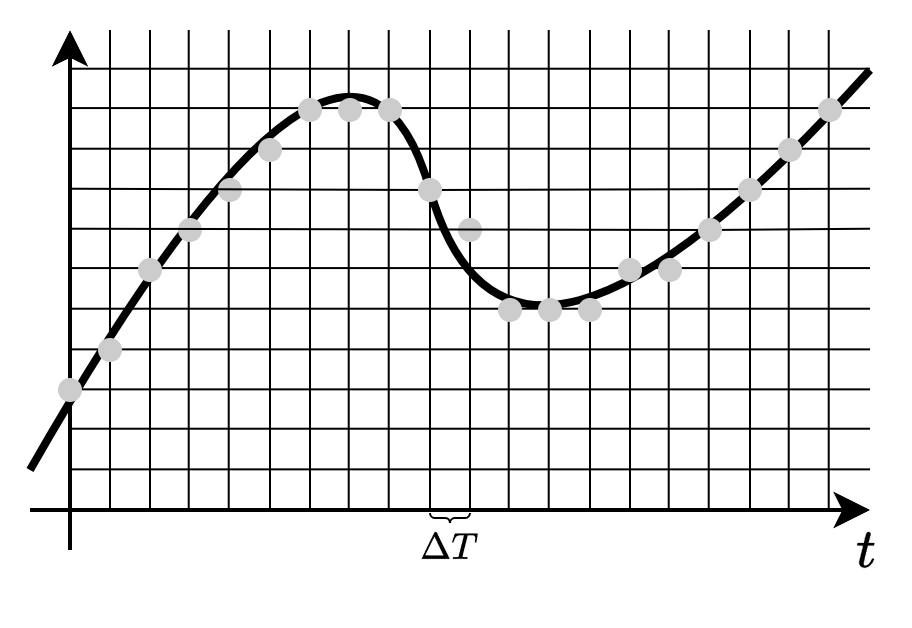
\includegraphics[width=0.5\linewidth]{images/discret1.png}
    \caption{Analog to digital conversion}
\end{figure}
The sampling frequency $f_S$ is the reciprocal of the sampling time $\Delta T$:
\[f_S=\dfrac{1}{\Delta T}\]
Here, $\Delta T$ represents the time discretization, while the amplitude discretization denotes the number of discrete levels available for conversion.
The effectiveness and cost of an ADC hinge on  $\Delta T$  (lower values being preferable) and the number of levels (higher values being desirable).

\paragraph*{Digital to analog converter}
The digital to analog converter (DAC) performs the conversion of digital signals into their analog counterparts, operating in the following manner:
\begin{figure}[H]
    \centering
    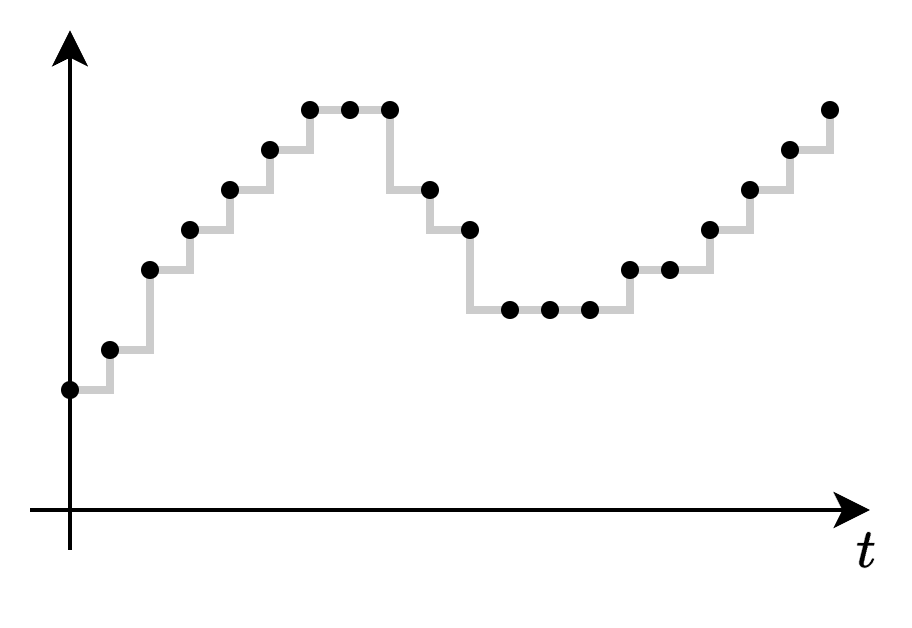
\includegraphics[width=0.5\linewidth]{images/discret2.png}
    \caption{Digital to analog conversion}
\end{figure}
The output signal from the DAC typically exhibits a step-like characteristic, known as zero-order-hold.
While higher-order hold techniques exist, they are less commonly employed in practical applications.

It's important to note that when the time interval $\Delta T$ between successive digital samples is sufficiently small, the step-like behavior becomes imperceptible or negligible.
Therefore, the quality of the DAC is primarily determined by the sampling time.